\documentclass[10pt,a4paper]{article}
\usepackage[margin=0.5in]{geometry}
\usepackage[utf8]{inputenc}
\usepackage{amsmath}
\usepackage{amsfonts}
\usepackage{amssymb}
\usepackage{natbib}
\bibliographystyle{plainnat}
\usepackage{hyperref}
\usepackage{graphicx}
\usepackage{subcaption}
\usepackage{booktabs}
\renewcommand{\arraystretch}{1.2}

\author{Claire Marie Guimond, Oliver Shorttle, John Rudge}
\title{Claire PhD Research Outline}

\begin{document}

\maketitle

\section{Steps}
\begin{enumerate}
\item Dynamic topography (key parameters---$a$, $M_p$, $q_{\rm stellar}$, $H_0$, $t_{\rm age}$, core mass fraction)
\begin{enumerate}
\item Steady state heat flux calculation as function of $a$, $M_p$, $X_{\rm K, U, Th}$
\item Thermal model

\begin{enumerate}

\item Steady-state isoviscous mantle
\item Temperature-dependent viscosity
\item Evolution with age
\item Realistic stagnant lid coupling
\end{enumerate}
\item Mapping temperatures to topography
\end{enumerate}

\item Flexural topography
\begin{enumerate}
\item Lithospheric strength model
\end{enumerate}

\item Things we wish we'd never thought of
\begin{enumerate}
\item Tidally-locked planets with non-uniform $T_s$, $T_m$
\item K/U/Th ratios vary depending on condensation history in protoplanetary disc; this introduces uncertainty... maybe look at stellar catalogues?
\end{enumerate}

\end{enumerate}

\section{Some simple calculations}

\subsection{Steady state heat flux}

We model a planet as a uniform sphere with mass $M_p$ and density $\rho$, and write energy balance equations for the surface and interior with fluxes in W.

At the surface, $Q_{\rm sfc}^{\uparrow} = Q_*^{\downarrow} + Q^{\uparrow}_{\rm bl}$, where $Q_{\rm sfc}^{\uparrow}$ is the blackbody radiation lost to space, $Q_*^{\downarrow}$ is the incident stellar flux, and $Q_{bl}$ is the flux from the interior from conduction across the boundary layer. The left hand side comprises outgoing fluxes, and the right hand side comprises incoming fluxes.

In the interior, the outgoing conductive flux across the boundary layer is balanced by internal radiogenic heating, $Q^{\uparrow}_{\rm bl} = Q_{\rm rad}$. If we don't know the boundary layer flux, which would depend on interior temperature, then
\begin{equation}
Q_{\rm sfc}^{\uparrow} = Q_*^{\downarrow} + Q_{\rm rad}.
\end{equation}

We can make order-of-magnitude estimations. First, the stellar contribution is parameterized as
\begin{equation}
Q_*^{\downarrow} = \frac{L_*(1-A)}{4a^2} \; \pi R_p^2,
\end{equation}
where $L_*$ is the stellar luminosity in W, $A$ is the planetary albedo, $a$ is the orbital semi-major axis in m, and $R_p = \left(\frac{3M_p}{4 \pi \rho}\right)^{1/3}$ is the radius of the planet. For a blackbody with 0 albedo,
\begin{equation}
Q_*^{\downarrow} = \frac{10^{26} \; {\rm W}}{\left(10^{11}\right)^2 \; \rm{m}^2} \cdot \left(\frac{10^{24}\;{\rm kg}}{10^3 \; {\rm kg}\;{\rm m}^3}\right)^{2/3} = 10^{17} \; {\rm W}.
\end{equation}


Next,
\begin{equation}
Q_{\rm rad} = \sum^{\rm K, U, Th}_n [ H_{0, n} \; X_n \; n_0 \; e^{-\ln 2 \frac{\tau}{\tau_{1/2 ,n}}} ] \; M_p,
\end{equation}
where we are summing over the heat-producing elements K, U, and Th, $H_{0, n}$ is the heat production of the $n^{th}$ isotope in W kg$^{-1}$, $X_n$ is the natural abundance of the $n^{th}$ isotope in terms of mass (compared to all isotopes of that element), $n_0$ is the concentration by mass of that element in the planet, $\tau$ is the age of the planet in seconds,  $\tau_{1/2 ,n}$ is the half-life of the $n^{th}$ isotope in seconds, and $M_p$ is the mass of the planet in kg. Using Earth values, and taking only the isotope with highest-order heat flux (40-K), we have
\begin{equation}
Q_{\rm rad} = \frac{10^{-5}\;{\rm W}}{{\rm kg}\;^{40}{\rm K}} \cdot \frac{10^{-3}\;\rm{kg\;K}}{\rm kg} \cdot \frac{10^{-4}\;{\rm kg}\;^{40}{\rm K}}{\rm{kg\;K}} \cdot 10^{24} \; {\rm kg} = 10^{12} \; {\rm W}.
\end{equation}

Therefore, $Q_{\rm sfc}^{\uparrow} = 10^{17} \; {\rm W} + 10^{12} \; {\rm W} = 10^{17} \; {\rm W}$.

To put this in terms of flux densities, we assume an isotropically-emitting sphere, so we have $q_{\rm sfc}^{\uparrow} = Q_{\rm sfc}^{\uparrow}/\rm{SA}_p$ where $\rm{SA}_p = 4\pi\;R_p^2$ is the of the planet's surface area, giving
\begin{equation}
q_{\rm sfc}^{\uparrow} = \frac{10^{17} \; {\rm W}}{10^1 \cdot \left(10^{24}\;{\rm kg}/10^3 \; {\rm kg}\;{\rm m}^3\right)^{2/3}} = 10^2 \; \rm{W\;m}^{-2}.
\end{equation}

\subsection{Thermal evolution of mantle with uniform viscosity and temperature}

The thermal state of a planetary mantle is controlled by the balance of heat loss (by conduction through the upper thermal boundary layer), $Q_{\rm ubl}$, with radiogenic heating, $Q_{\rm rad}$. Secular core cooling represents an additional source of heat to the mantle, here represented by an optional parameter. In this section we make the preliminary simplifying assumption that viscosity does not change with temperature.

The change in temperature due to this balance is governed by the O.D.E.,
\begin{equation}
M_m c_v \frac{{\rm d}T_m}{{\rm d}t} = -Q_{\rm ubl} + Q_{\rm rad} + Q_{\rm CMB},
\end{equation}
where $M_m$ is the mantle mass, $c_v$ is the mantle specific heat capacity at constant volume, $Q$ is the integral of the heat flux over surface area or volume, respectively, and the sign of $Q$ indicates cooling or heating. We use {\tt scipy.integrate} to integrate this O.D.E. from $\tau_0$, taken to be the time of magma ocean cooling, until the age of the planet, $\tau_f$.  

\begin{table}
\label{tab:params}
\end{table}

Table \ref{tab:params} lists the free parameters in this model, being the planetary mass, $M_p$, semi-major axis, $a$, and core mass fraction, CMF; as well as the stellar luminosity, $L_*$, planetary albedo, Alb, mantle thermal conductivity, $k_m$, mantle thermal expansivity, $\alpha_m$, mantle density, $\rho_m$, mantle heat capacity at constant volume, $c_v$, critical Rayleigh number for convection, Ra$_{\rm crit}$, and mantle dynamic viscosity, $\eta_m$, along with the radioisotope parameters described above.

From this we also calculate a number of derived parameters:

the radius of the planet, $R_p$, based on \citet{Zeng2016} using PREM,
\begin{equation}
\frac{R_p}{R_E} = (1.07 - 0.21\; {\rm CMF})\left(\frac{M_p}{M_E}\right)^{1/3.7},
\end{equation}
which has surface area SA$_p$; the radius of the core, using the scaling relationship from \citet{Zeng2017},
\begin{equation}
R_c = R_p \; {\rm CMF}^{0.5},
\end{equation}
which has surface area SA$_c$; the surface gravity,
\begin{equation}
g_{\rm sfc} =\frac{6.674\times 10^{-11}M_p}{R_p^2};
\end{equation}
the surface temperature, $T_s$, assuming the surface is in blackbody equilibrium,
\begin{align}
T_s &= \left(\frac{q_* \pi R_p^2}{\sigma \; {\rm SA}_p}\right)^{1/4},\\
q_* &= \frac{L_*(1-{\rm Alb})}{4 \pi a^2};
\end{align}
the thermal diffusivity of the mantle,
\begin{equation}
\kappa_m = \frac{k_m}{\rho_m c_p};
\end{equation}

A vigorously-convecting medium is said to be isothermal except in its upper and lower boundary layers, which have steep temperature gradients.  Heat escapes the system via conduction through the boundary layers. For mantle thermal evolution, we only consider heat transport through the upper boundary layer. Hence mantle cooling depends on the boundary layer thickness, $d_{\rm lid}$, as well as the temperature difference between the mantle and surface, $\Delta T = T_m - T_s$, and the thermal conductivity of the mantle, $k_m$:
\begin{align}
Q_{ubl} &= \int_{\rm A} q_{ubl} \; {\rm d}A = q_{ubl} \; {\rm SA}_p,\\
q_{ubl} &= \frac{k_m \Delta T}{\delta_{ubl}}.
\label{eq:q_ubl}
\end{align}
$\delta_{ubl}$ is calculated by setting the Rayleigh number to its critical value for initiating convection:
\begin{equation}
\delta_{ubl} = \left(\frac{{\rm Ra}_c \eta_m \kappa_m}{\alpha_m \rho_m g_{\rm sfc} \Delta T}\right)^{\frac{1}{3}}
\label{eq:d_ubl}
\end{equation}

Meanwhile, radiogenic heating is the same as in the previous section:
\begin{align}
Q_{\rm rad} &= \int_{M_p} q_{\rm rad} \; {\rm d}M = q_{\rm rad} M_p,\\
q_{\rm rad} &= \sum^{\rm K, U, Th}_n \left[ H_{0, n} \; X_n \; n_0 \; e^{-\ln 2 \frac{\tau}{\tau_{1/2 ,n}}} \right],
\end{align}

If CMF \textgreater \; 0, then the heat flux across and thickness of the lower thermal boundary layer of the mantle is obtained by analogy to equations \ref{eq:q_ubl} and \ref{eq:d_ubl}, where $\Delta T = T_c - T_m$, $\delta_{ubl}$ is replaced by lower boundary layer thickness $\delta_{lbl}$ with gravity evaluated at $R_c$.

%\begin{equation}
%{\frac{{\rm d}T_m}{{\rm d}t}}_{\rm rad} = \frac{h [{\rm W} \; {\rm kg}^{-1}] \times M_m [{\rm kg}]}{M_m [{\rm kg}] \times c_v [{\rm J}\;{\rm kg}^{-1}\;{\rm K}^{-1}]} = \frac{{\rm K}}{{\rm s}}
%\end{equation}

\subsection{Thermal evolution of a stagnant lid planet}

So far, we have not distinguished between the upper thermal boundary layer of the mantle and the stagnant lid. This is important because the stagnant lid may have a different temperature profile than the convecting mantle, with different internal heating rates. In reality the temperature at the top of the mantle thermal boundary layer, $T_l$, would not be set at the planetary surface temperature. To find the radius $R_l$ at which we find $T_l$, we use continuity of temperature.

Fluid dynamics experiments show that the temperature jump, $\Delta T_{ubl}$, between the isothermal core at $T_m$ and the top of the thermal boundary layer at $T_l$ is proportional to the ``viscous temperature scale" $\Delta T_\eta$, the rate of viscosity change with temperature \citep{DavailleJaupart1993}. Following the method of \citet{Thiriet2019}, $\Delta T_{ubl}$ is a function of only the isothermal core temperature:
\begin{align}
\label{eq:Tl}
\Delta T_{ubl} &= -a_{rh} \Delta T_{\eta} \\
\Delta T_{\eta} &= \frac{\eta(T_m)}{{\rm d}\eta/{\rm d}T_m\vert_{Tm}} = \frac{R_b T_m^2}{E_a},
\end{align}
Here, $R_b$ is the universal gas constant, and $a_{rh} = 2.54$ based on fits to 3D convection models \citep{Thiriet2019}. $E_a$ is the activation energy in the Arrhenius law for viscosity as a function of temperature:

\begin{equation}
\eta(T_m) = \eta_0 \; {\rm exp}\left[\frac{E_a}{R_b}\left(\frac{1}{T_m} - \frac{1}{T_0}\right)\right],
\end{equation}
where $\eta_0$ and $T_0$ are the reference viscosity and temperature.

In the stagnant lid of thickness $d_l$ above this layer, the temperature decreases from $T_l = T_m + \Delta T_{ubl}$ to $T_s$ by conductive heat transport. As on Earth, there may be different internal heating rates in this layer than in the mantle; the temperature profile in figure \ref{fig:T_z} is:
\begin{equation}
T_{\rm lid}(z) = \frac{-H_l}{2k}z^2 - \frac{q_{ubl} +d_l H_l}{k}z + T_s,
\end{equation}
where the $z$-axis points perpendicularly upwards from the surface, $z=0$. $H_l$ is the lithospheric heat production in W m$^{-3}$, assumed to be constant with $z$ at a given time step for simplicity. This is the standard solution for steady-state heat conduction with internal heating, where $q(z=0) = q(z=-\Delta z) + H \Delta z$.

%\begin{figure}
%\centering
%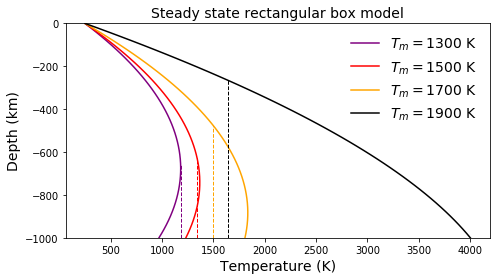
\includegraphics[width=0.7\textwidth]{../T_z.png}
% \caption{Thermal profile in the lithosphere for different mantle temperatures $T_m$ (coloured lines). Dashed lines show the temperature at the lid base from equation \ref{eq:Tl} for that mantle temperature. \label{fig:T_z}}
%\end{figure}

At intermediate complexity, we assume temperature is continuous where the upper thermal boundary layer meets the stagnant lid:
\begin{align}
\label{eq:t-continuity}
&T_{\rm lid}(z=-d_l) = T_m + \Delta T_\eta \\
&\frac{H_l}{2k}d_l^2 + \frac{q_{ubl}\left(T_m\right)}{k}d_l + \left(T_m - T_s - \frac{R_b}{E_a}T_m^2\right)  = 0
\end{align}
where $q_{ubl}$ is a function of only $T_m$ if $\beta=1/3$ ($\delta_{ubl}$ independent of mantle depth). The roots of this equation give $d_l$ as a function of $T_m(t)$ and $H_l(t)$, which allows $d_l$ to be calculated at each time-step. It can be shown that there is one positive root for our range of parameters.

We can use {\tt sympy} to write an analytic expression for $d_l$ in terms of $T_m$, although it's quite long. Figure \ref{fig:d_fT} plots this for different values of $H_l$, showing that for our choice of parameters, $d_l$ peaks around $T_m = 1400$~K.

%\begin{figure}
%\centering
%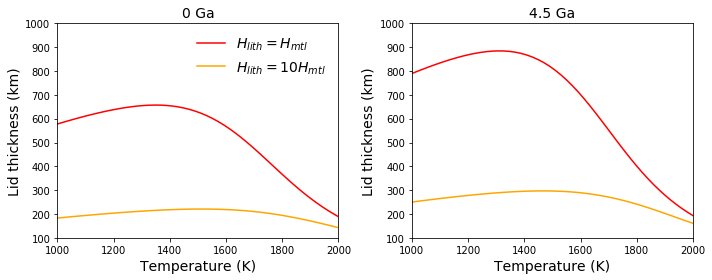
\includegraphics[width=\textwidth]{../d_T.png}
% \caption{Lid thickness as a function of mantle temperature for different radiogenic heating rates in the lithosphere: either equal to the mantle value (red line), or $10\times$ the mantle value (orange line). \label{fig:d_fT}}
%\end{figure}

Results for the thermal evolution of a 1-Mars mass planet using this stagnant lid parameterization are shown in figure \ref{fig:evol-lid}.

%\begin{figure}
%\includegraphics[width=\textwidth]{../figs/evol.png}
%\caption{Thermal evolution of a 1-Mars mass planet, using the input values of \citet{Thiriet2019}, and assuming that the radiogenic element abundance in the lithosphere is equal to that of the mantle. Results for the lid thickness may be compared to figure \ref{fig:thiriet-lid}. \label{fig:evol-lid}}
%\end{figure}
%
%\begin{figure}
%        \includegraphics[width=\textwidth]{../figs/thiriet.png}
%        \caption{Stagnant lid evolution from \citet{Thiriet2019}. From their paper: {\footnotesize ``The stagnant lid thickness evolution obtained for Mars’s 3-D model is shown in blue: in (a) if the base of the lid is defined by the intersection between the tangent to the velocity profile at the depth corresponding to the maximum velocity gradient and the radius axis (method 1, Reese et al., 2005), in (b) if it corresponds to the depth where 1\% of the maximum velocity is reached (method 2). We obtain best fits when considering in 1-D models $u$ = 0.345 $a_{rh}$ = 2.16 for method 1 and $u$ = 0.338 $a_{rh}$ = 2.32 for method 2 (red dotted dashed lines). Stagnant lid thickness evolution for 1-D models are also shown for some of our best scaling parameter combinations $u$ = 1/3 and $a_{rh}$ = 2.44 (green
%dashed lines), $u$ = 1/4 and $a_{rh}$ = 5.3 (black dashed lines) and $u$ = 0.335 and $a_{rh}$ = 2.54 (our best combination for the three planets, red solid lines)."} \label{fig:thiriet-lid}}
%\end{figure}



\subsection{Viscous stress and topography}

Stress has units of force over area

We can use this simple relation to estimate dynamic topography in terms of heat flow and temperature. The shear stress associated with a rising or sinking plume (a density difference) in the interior is given by:

\begin{align}
\sigma_{rr} &\propto \rho g \alpha \Delta T_{rh} \delta_{bl} \\
&= C \rho_m \alpha_m g \left(\frac{R_b T_m^2}{E_a}\right)^2 \frac{k_m}{q_{bl}},
\end{align}
which is the volume change due to a temperature change, where the expressions \ref{eq:Tl} and \ref{eq:d_ubl} are substituted for $\Delta T_{rh}$ and $\delta_{bl}$. \citet{Reese2005} give $C = 0.1$ for interior stress and $C = 2$ for lid stress.

At equilibrium, this stress is balanced by the downwards gravitational force of a topographic load, $\sigma_{rr} = \rho g h$, where $h$ is the amplitude of topography. Thus, in this simple force balance, $h$ scales with $T_m$ and $q_{bl}$ as:
\begin{equation}
h = C \alpha \left(\frac{R_b T_m^2}{E_a}\right)^2 \frac{k_m}{q_{bl}}
\end{equation}

Confused - shear stress or normal stress in balace?

\subsubsection{Observations of dynamic topography in the solar system}

This analysis results in values for dynamic topography which are rather far off from what is seen in the solar system. Table \ref{tab:dyn_topo_obvs} compiles these observations for Venus and Mars. Note that Earth's dynamic topography is made more complex by, e.g., subducting plates, and is not focussed on here, although a sample of values is presented for comparison.\\

\begin{tabular}{@{} l r r r r p{3cm} @{}} \label{tab:dyn_topo_obvs}
\toprule
Reference & RMS (km) & Amplitude (km) & $l=2$ power (km) & Heat flow (mW m$^{-2}$) & Notes \\
\midrule
\textbf{Mars} & & & & \\
\citet{Golle2012} & & & & & Cannot compare to actual Mars because signal would be dominated by Tharsis rise, only show geoid \\

\midrule
\textbf{Venus} & & & & \\

\citet{Solomatov1996} & ? & $\sim$3 & & & Topography from ``thermal thinning" \\
\citet{Huang2013} & & & $\sim$1 & &  \\
\citet{Golle2012} & & & 3.3 & & Result without elastic lid \\
\citet{Yang2016} & ? & $\sim$3 & & & Separated dynamic and isostatic components \\

\midrule
\textbf{Earth} & & & & \textbf{37\textendash 41 TW} & \citet{Jaupart2007} \\
\citet{Arnould2018} & 3.47\textendash 7.28 & & & 6.9\textendash 83 TW & 2D numerical models \\
\citet{Amante2009} & 2.17 & & & & \\
\citet{Pari2001} & & 0.2 & & & 1st degree spherical hamonic \\
\citet{Kiefer1998} & & & & & Given non-dimensionalized, need to convert \\



\bottomrule
\end{tabular}



\bibliography{exogeodynamics}


\end{document}

